\chapter{Simulaci\'on de la emisi\'on de radio de las EAS}
\label{ch:simulacionRadio}

\section{ZHAireS}

\zhs{} es una implementaci\'on del las rutinas de ZHS \cite{1_halzen_zas_stanev_1991,2_zas_halzen_stanev_1992} sobre \aires{} desarrollada por Jaime Alvarez-Muñiz, Washington Rodriguez-Carvhalo Jr. y Matias Tueros en el Departamento de Física de Partículas Universidad de Santiago de Compostela, España.
Una vez instalado \zhs{} se conservan todas las capacidades de \aires{} y s\'olo se agrega la posibilidad de simular el la emisi\'on de radio de la EAS, incluyendo nuevas directivas de entrada que permiten controlar con buen detalle la simulacion.

	\subsection{C\'omputo de la se\~nal}
	
	La metodolog\'ia aplicada en \zhs{} para calcular la se\~nal es simple: cada vez que el algoritmo de \aires{} avanza una part\'icula se llama las rutinas de ZHS para calcular el pulso electromagn\'etico que esta generar\'ia en ciertos observadores (o antenas) que se ubican en posiciones predefinidas.
	Esto se esquematiza en la figura \ref{fig:trackSch}.
	
	\begin{figure}[ht!]
	\centering
		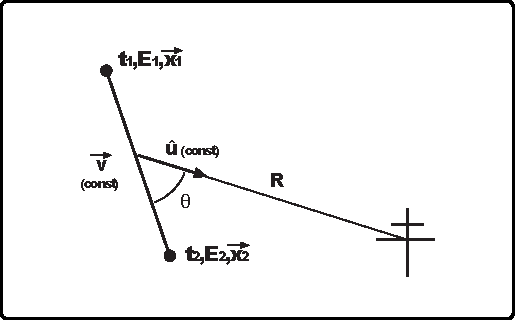
\includegraphics[width=0.6\textwidth]{fig/simulacionRadio/trackSch}
		\caption{\label{fig:trackSch} Esquema del track que avanza una par\'icula al ser simulada por \aires{}.}
	\end{figure}
	
	Dado que el c\'alculo exacto de la emisi\'on electromagn\'etica de una part\'icula que se desplaza con velocidad constante en cierto camino involucra la resoluci\'on num\'erica de un par de integrales, las rutinas de ZHS utilizan una aproximaci\'on que salva este problema a costa de cumplir las siguientes hip\'otesis:
	\begin{enumerate}
	 \item El observador se encuentra en la zona de campo lejano
	 \begin{equation}
	  kr\gg1
	 \end{equation}
	 \item La longitud del track es peque\~na a comparaci\'on de la distancia al observador, $\eta\ll1$, con
	 \begin{equation}
	  \eta = \frac{k L^2}{R}\sin^2\theta
	 \end{equation}
	 donde $L\equiv v(t_1-t_2)$ es la longitud del track.
	 \item La inversa distancia entre cualquier punto del track y el observador debe poder ser considerada una constante
	 \begin{equation}
	  \frac{1}{r(t)}\sim\frac{1}{R}
	 \end{equation}
	\end{enumerate}
	Si el tama\~no de los tracks obtenidos a partir del algoritmo de \aires{} no siatisface alguna de las condiciones 2 o 3, una rutina se encarga de partirlo en trozos lo suficientemente chicos como para que esto suceda.
	Si no se llegara a cumplir la condici\'on n\'umero 1, ser\'ia necesario utilizar la resoluci\'on exacta del problema, lo que no se encuentra implementado en \zhs{} hasta el momento.
	Esta es una limitaci\'on conocida del c\'odigo, que genera se\~nales artificiales en las antenas, aunque la probabilidad de que esto ocurra es muy baja incluso en EAS que se desarrollan muy cerca del detector como las iniciadas por neutrinos earth-skimming.
	
	Una vez que los tracks cumplen la scondiciones necesarias, se calcula el potencial vector $\vec{A}(t,\hat{u})$ y el campo el\'ectrico $\vec{E}(t,\hat{u})$ en la posici\'on del observador utilizando las ecuaciones \ref{eq:afield} y \ref{eq:efield}.
	\begin{equation}
	\vec{A}(t,\hat{u})
	=
	\frac{\mu e}{4\pi Rc}
	\vec\beta_{\bot}
	\frac{\Theta(t-t^{det}_1)-\Theta(t-t^{det}_2)}{1-n\vec\beta\cdot\hat u}
	\label{eq:afield}
	\end{equation}
% 	$\vec E(t)=-\partial\vec{A}/\partial t $
	\begin{equation}
	\vec{E}(t,\hat{u})
	=
	-\frac{\mu e}{4\pi Rc}
	\vec\beta_{\bot}
	\frac{\delta(t-t^{det}_1)-\delta(t-t^{det}_2)}{1-n\vec\beta\cdot\hat u}
	\label{eq:efield}
	\end{equation}
	En estas, como en la figura \ref{fig:trackSch}, $\hat{u}$ es el versor que indica la direcci\'on entre la mitad del track y el observador, $\vec\beta=\vec v/c$, $\vec\beta_{\bot}=-[\hat{u}\times(\hat{u}\times\vec\beta)]$ es la proyecci\'on de $\vec\beta$ sobre el plano perpendicular a $\hat u$ y $t_{1,2}^{det}=t_{1,2}+nR/c-n\vec\beta \cdot \hat u (t_{1,2}-t_0)$ son los tiempos de detecci\'on del principio y final del track respectivamente, con $t_0=(t_1+t_2)/2$. Por otro lado, $\Theta(x)$ y $\delta(x)$ son las funciones de escalon de Heaviside y delta de Dirac respectivamente.
	
	Para realizar un c\'alculo correcto del tiempo de arrivo de la se\~nal a la antena, es necesario tener en cuenta el \'indice de refracci\'on de la atm\'osfera como se especifica en la ecuaci\'on \ref{eq:refIndexEff}.
	\begin{equation}
		\begin{matrix}
		n_{eff}
		=
		1+{\mathcal R}_{eff}\times10^{-6}
		&
		{\rm con}
		&
		{\mathcal R}_{eff}
		=
		\frac{1}{R}\int_0^R{\mathcal R}(h)dl
		\end{matrix}
	\label{eq:refIndexEff}
	\end{equation}
	donde ${\mathcal R}(h) = \left[ n(h)-1 \right] \times 10^6$.
	Para ${\mathcal R}(h)$ \zhs{} ofrece la posibilidad de utilizar un valor constante, o un modelo exponencial como el de la ecuaci\'on \ref{eq:refIndexExp}
	\begin{equation}
	{\mathcal R}(h)
	=
	{\mathcal R}_o
	exp(-K_rh)
	\label{eq:refIndexExp}
	\end{equation}
	en el que ${\mathcal R}_o={\mathcal R}(h=0)\equiv 325$ y $K_r=0.1218km^{-1}$.
	Con estos valores es posible reproducir los valores calculados en \cite{gerson1948polar} con un $1\%$ precisi\'on hasta una altura de \cant{10}{km}.
	A mayor altitud la aproximaci\'on exponencial para ${\mathcal R}$ sobreestima el \'indice de refracci\'on, pero m\'as all\'a de los 20km la lluvia recien ha comenzado a desarrollarse, por lo que la cantidad de part\'iculas es relativamente peque\~na por lo que esta zona contribuye muy poco a la se\~nal total.
	
	Otro factor a tener en cuenta es que cuando las lluvia a simular es muy inclinada, la altura que se utiliza en la ecuaci\'on \ref{eq:refIndexExp} debe ser medida desde la superficie de la tierra, sin utilizar la aproximai\'on de tierra polana, como se muestra en la figura \ref{fig:refIndex}.
	\begin{figure}[ht!]
	\centering
		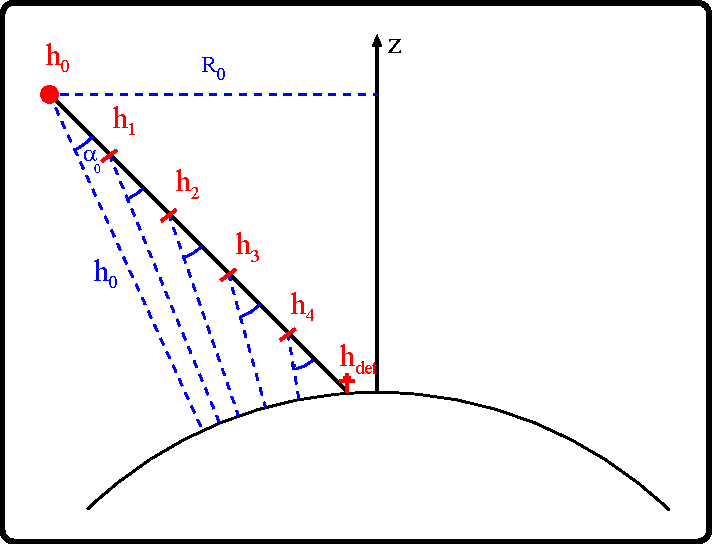
\includegraphics[width=0.6\textwidth]{fig/simulacionRadio/refIndex}
		\caption{\label{fig:refIndex} Esquema del m\'etodo mediante el que se tiene en cuenta la curvatura de la tierra al momento de calcular el \'indice de refracci\'on de la atm\'osfera para diferentes alturas.}
	\end{figure}
	dado que realizar la integral descripta en \ref{eq:refIndexEff} en estas condiciones es muy costoso, se discretiza $R$ en un n\'umero finito de tramos y supone el \'indice de refracci\'on constrante en cada uno de ellos.
	
	Una vez calculadas las amplitudes de los campos y los tiempos de arrivo de las se\~nales debidas a cada track, el campo total en cada observador se guarda utilizando bines temporales prefijados, como la ecuaci\'on \ref{eq:eAntField}, donde el \'indice $j$ corre sobre las part\'iculas simuladas y $\omega_j$ es el peso estad\'istico que pose\'ia la part\'icula que emiti\'o el campo $\vec{E}_j$.
	\begin{equation}
	\vec{E}(t_i)=\sum_{j:t_j\varepsilon[t_i,t_{i+1}]}\vec{E}_j(t_j)\omega_j
	\label{eq:eAntField}
	\end{equation}
	
	La ecuaci\'on \ref{eq:eAntField} muestra claramente que la se\~nal simulada en una dada antena depende fuertemente del algoritmo de thinning utilizado. 
	Dado que, como se ver\'a en la secci\'on de resultados, la mayor contribuci\'on al campo el\'ectrico proviene de las part\'iculas de media y baja energ\'ia, es poco deseable la aparici\'on de pesos extremadamente altos.
	En consecuencia y como bajar el nivel de thinning es poco eficiente, lo que se recomienda es utilizar un \emph{weight factor} peque\~no.

\section{Caracterizaci\'on de eventos ES}
	
	\subsection{Caracter\'isticas generales}
	
	
	\begin{figure}[ht!]
		\centering
		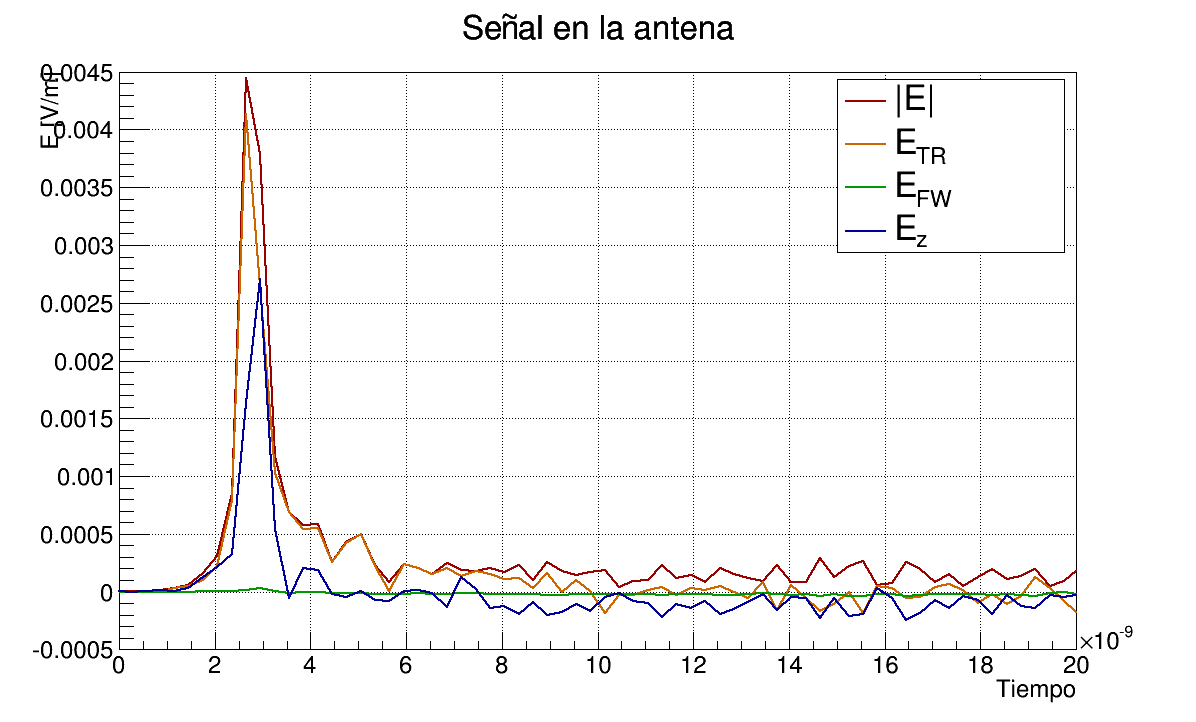
\includegraphics[width=0.8\textwidth]{./fig/simulacionRadio/antennaSignal.png}
		\caption{\label{fig:antSig}
		asd
		}
	\end{figure}
	
	En la figura \ref{fig:testFootprint_E0} se muestra la se\~nal de radio en el suelo para una lluvia simulada en Malarg\"ue, cuyos par\'ametros de simulaci\'on se resumen en la tabla \ref{tab:paramTestShower}
	
	\begin{table}[ht!]
	 \begin{center}
	  \begin{tabular}{ccccc}
	   Canal de decaimiento & $E_v$ & $\theta$ & \xd{} & $\phi$ \\
	   \hline
	   $\tau\rightarrow e^- \nu_{e^-}\nu\tau$ & \cant{10^{18}}{eV} & \cant{90.5}{^\circ} & \cant{25}{m} & \cant{90}{^\circ}
	  \end{tabular}
	  \caption{\label{tab:paramTestShower}
	  as
	  }
	 \end{center}
	\end{table}

	
	\begin{figure}[ht!]
		\centering
		\includegraphics[width=\textwidth]{./fig/simulacionRadio/{foorPrint_ZWv1.22_ntuples_v1.21_ChTest_phi_90_18_89.5_90_25_1238_E0}.png}
		\caption{\label{fig:testFootprint_E0}
		asd
		}
	\end{figure}
	
	\begin{figure}[ht!]
		\centering
		\includegraphics[width=\textwidth]{./fig/simulacionRadio/{foorPrint_ZWv1.22_ntuples_v1.21_ChTest_phi_90_18_89.5_90_25_1238_E0x}.png}
		\caption{\label{fig:testFootprint_E0tr}
		asd
		}
	\end{figure}
	
	\begin{figure}[ht!]
		\centering
		\includegraphics[width=\textwidth]{./fig/simulacionRadio/{foorPrint_ZWv1.22_ntuples_v1.21_ChTest_phi_90_18_89.5_90_25_1238_E0y}.png}
		\caption{\label{fig:testFootprint_E0fw}
		asd
		}
	\end{figure}
	
	\begin{figure}[ht!]
		\centering
		\includegraphics[width=\textwidth]{./fig/simulacionRadio/{foorPrint_ZWv1.22_ntuples_v1.21_ChTest_phi_90_18_89.5_90_25_1238_E0z}.png}
		\caption{\label{fig:testFootprint_E0z}
		asd
		}
	\end{figure}
	
	\subsubsection{Emisi\'on coherente - Cono \cher}
	
	\begin{figure}[ht!]
		\centering
		\includegraphics[width=\textwidth]{./fig/simulacionRadio/{foorPrint_Cone_ZWv1.22_ntuples_v1.21_ChTest_phi_90_18_89.5_90_25_1238_E0}.png}
		\caption{\label{fig:testFootprint_Cone}
		asd
		}
	\end{figure}
	
	\clearpage
	\subsection{Tratamiento de la se\~nal}
	
	\begin{figure}[ht!]
		\centering
		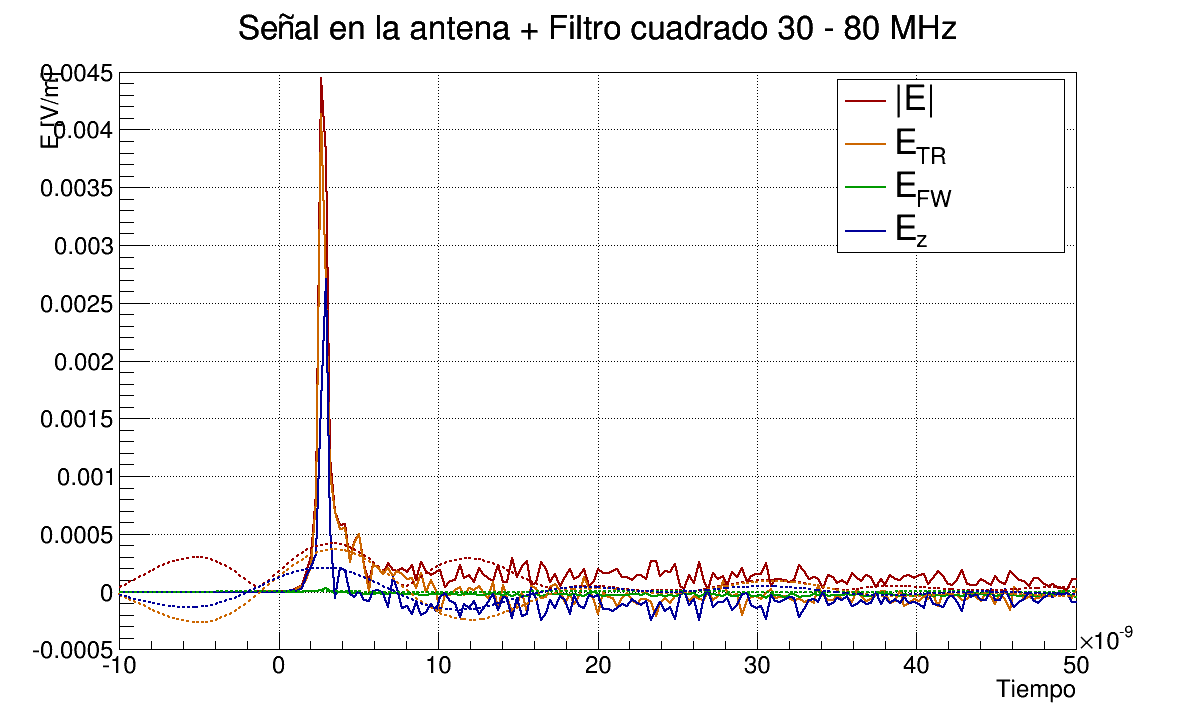
\includegraphics[width=0.8\textwidth]{./fig/simulacionRadio/antennaFilt.png}
		\caption{\label{fig:antFilt}
		asd
		}
	\end{figure}
	
	\begin{figure}[ht!]
		\centering
		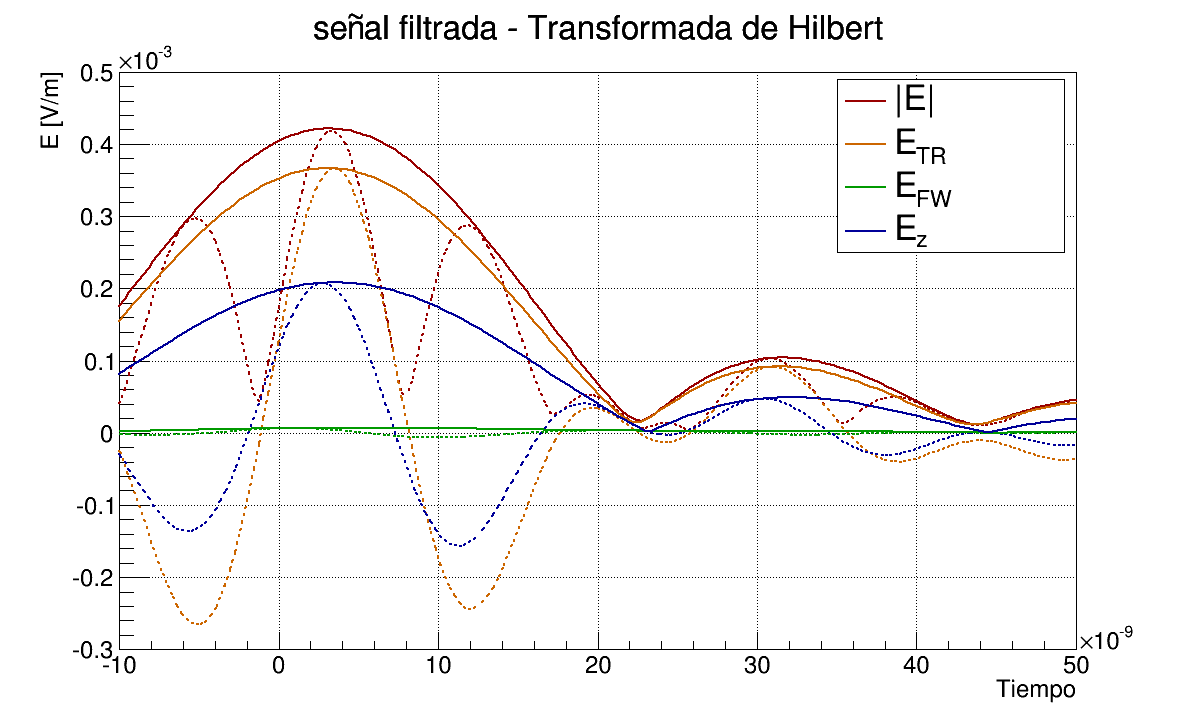
\includegraphics[width=0.8\textwidth]{./fig/simulacionRadio/antennaHEnv.png}
		\caption{\label{fig:antHEnv}
		asd
		}
	\end{figure}
	
	
	\begin{figure}[ht!]
		\centering
		\includegraphics[width=\textwidth]{./fig/simulacionRadio/{foorPrint_ZWv1.22_ntuples_v1.21_ChTest_phi_90_18_89.5_90_25_1238_E}.png}
		\caption{\label{fig:testFootprint_E}
		asd
		}
	\end{figure}
	
	\begin{figure}[ht!]
		\centering
		\includegraphics[width=\textwidth]{./fig/simulacionRadio/{foorPrint_ZWv1.22_ntuples_v1.21_ChTest_phi_90_18_89.5_90_25_1238_Ex}.png}
		\caption{\label{fig:testFootprint_Etr}
		asd
		}
	\end{figure}
	
	\begin{figure}[ht!]
		\centering
		\includegraphics[width=\textwidth]{./fig/simulacionRadio/{foorPrint_ZWv1.22_ntuples_v1.21_ChTest_phi_90_18_89.5_90_25_1238_Ey}.png}
		\caption{\label{fig:testFootprint_Efw}
		asd
		}
	\end{figure}
	
	\begin{figure}[ht!]
		\centering
		\includegraphics[width=\textwidth]{./fig/simulacionRadio/{foorPrint_ZWv1.22_ntuples_v1.21_ChTest_phi_90_18_89.5_90_25_1238_Ez}.png}
		\caption{\label{fig:testFootprint_Ez}
		asd
		}
	\end{figure}
	
	\clearpage
	\subsection{Evoluci\'on de la se\~nal a nivel del suelo}
		
	
	mostrar evolucion del EMax a lo largo de la lluvia
	
	mostrar espectro y evolucion
	
	mostrar fit del maximo de la lluvia como funcion de xd y theta y dependencia con la energia
	
		\subsubsection{Evoluci\'on de la polarizaci\'on}
		
		cambio askaryan geomagnetico?
	
	\subsection{Corte en $\theta$}
	
	plots dado xd para diferentes thetas
	mostrar tomataso
	
	\clearpage
	\subsection{Influencia del campo magn\'etico terrestre}
	
	\begin{figure}[ht!]
		\centering
		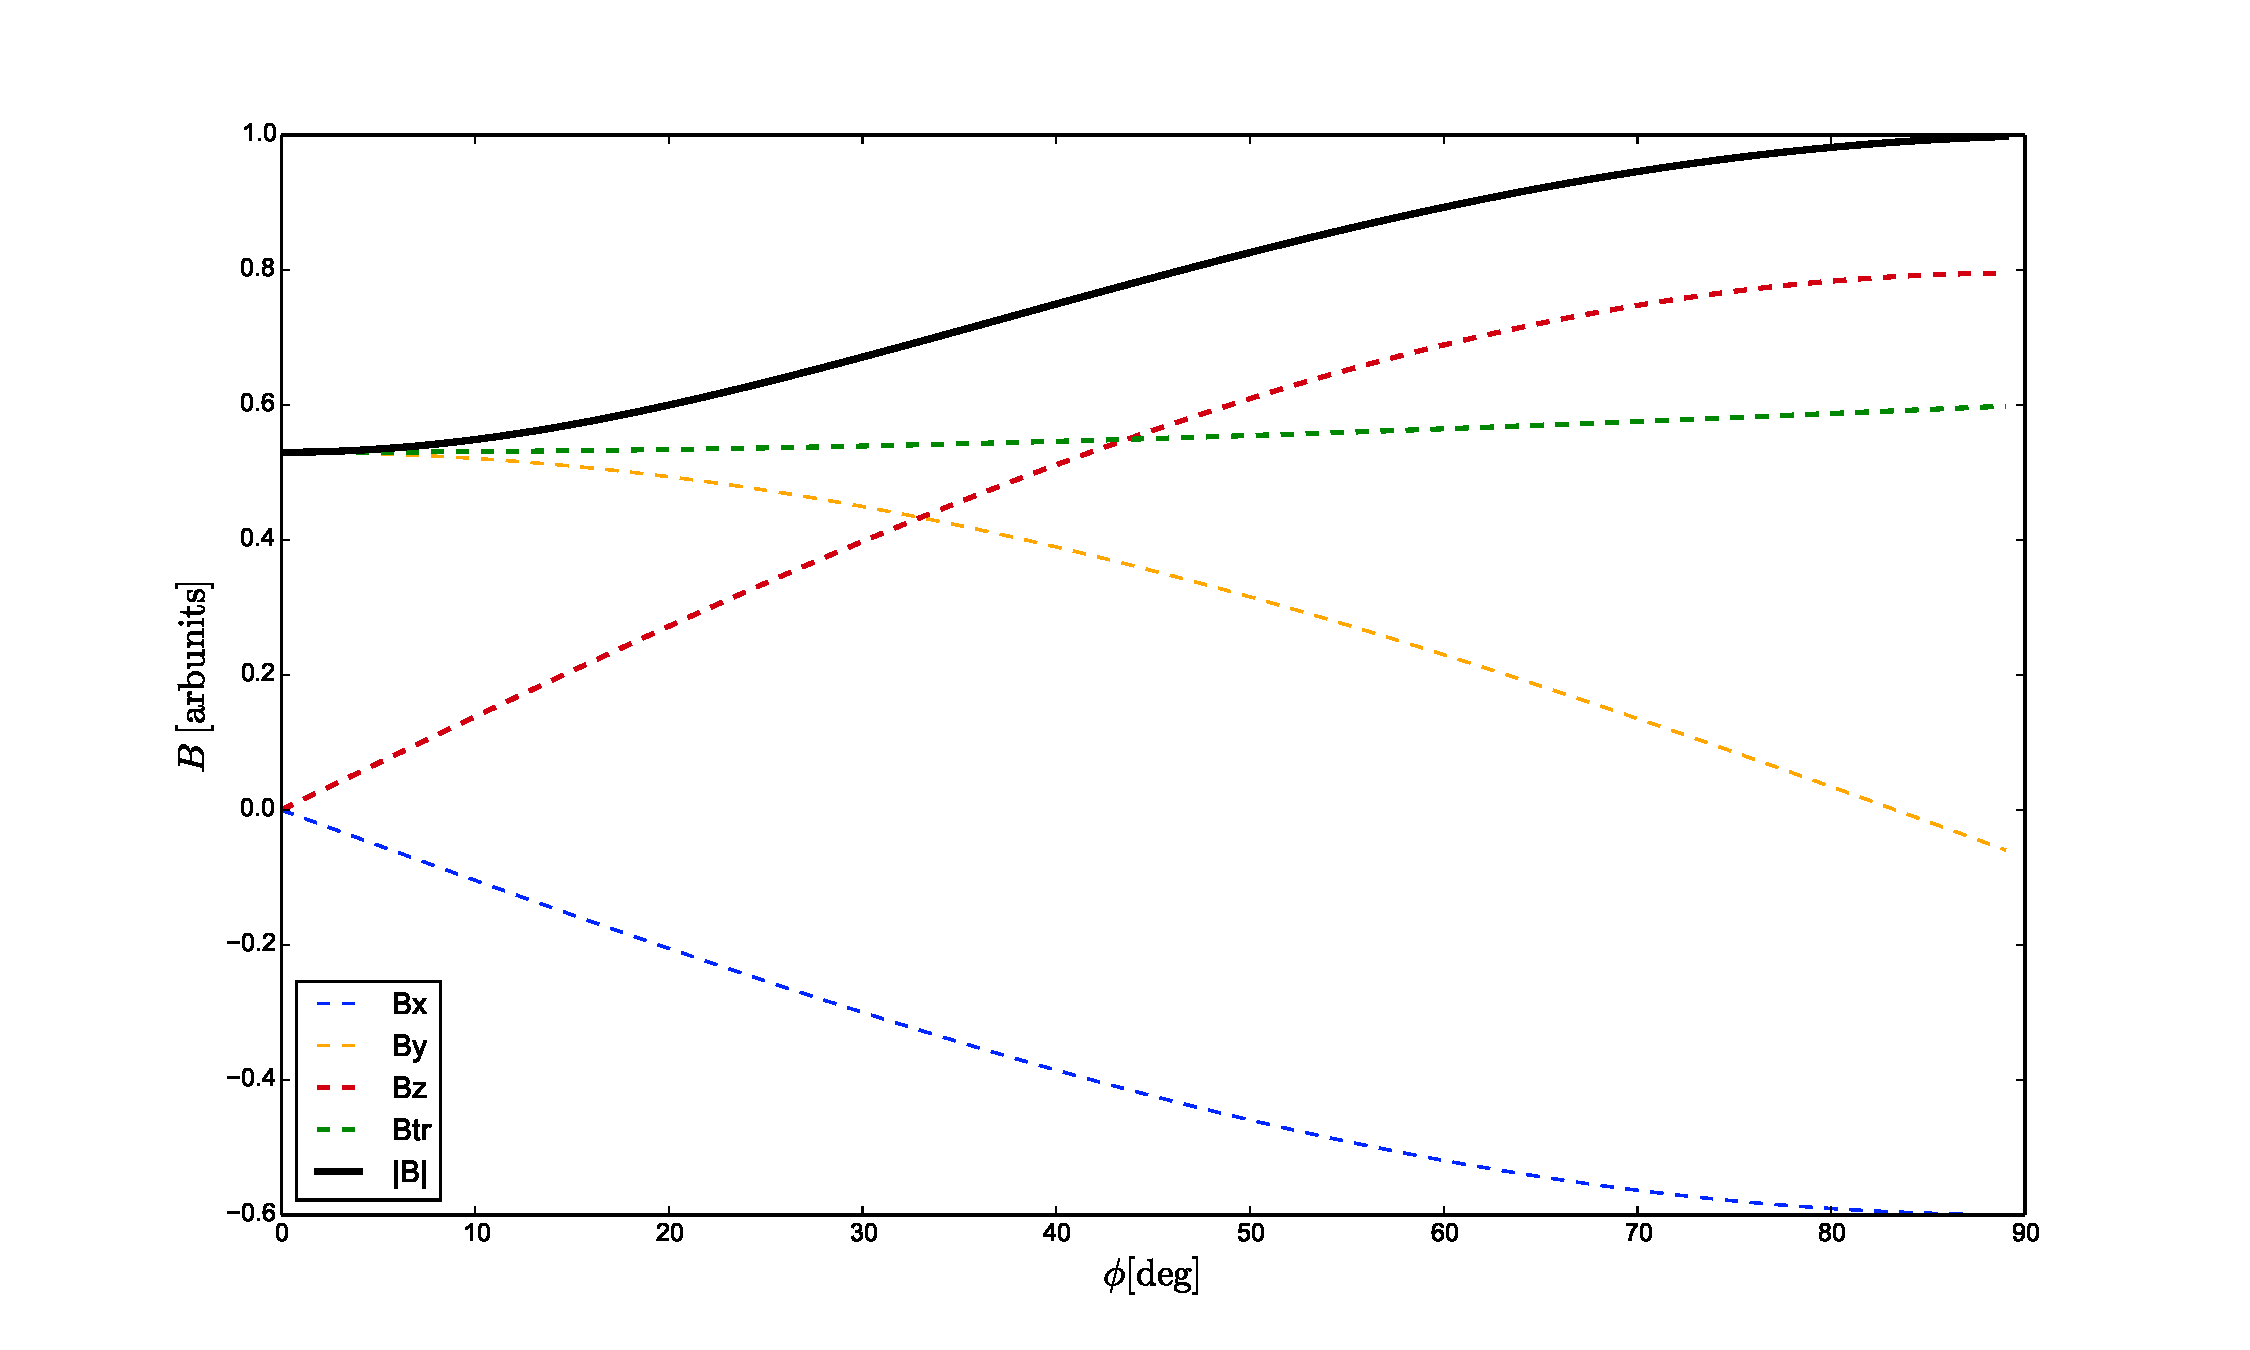
\includegraphics[width=\textwidth]{./fig/EASRadio/geomComps_Malarge}
		\caption{\label{fig:geomComps_Malarge}
		asd
		}
	\end{figure}
	
	\begin{figure}[ht!]
		\centering
		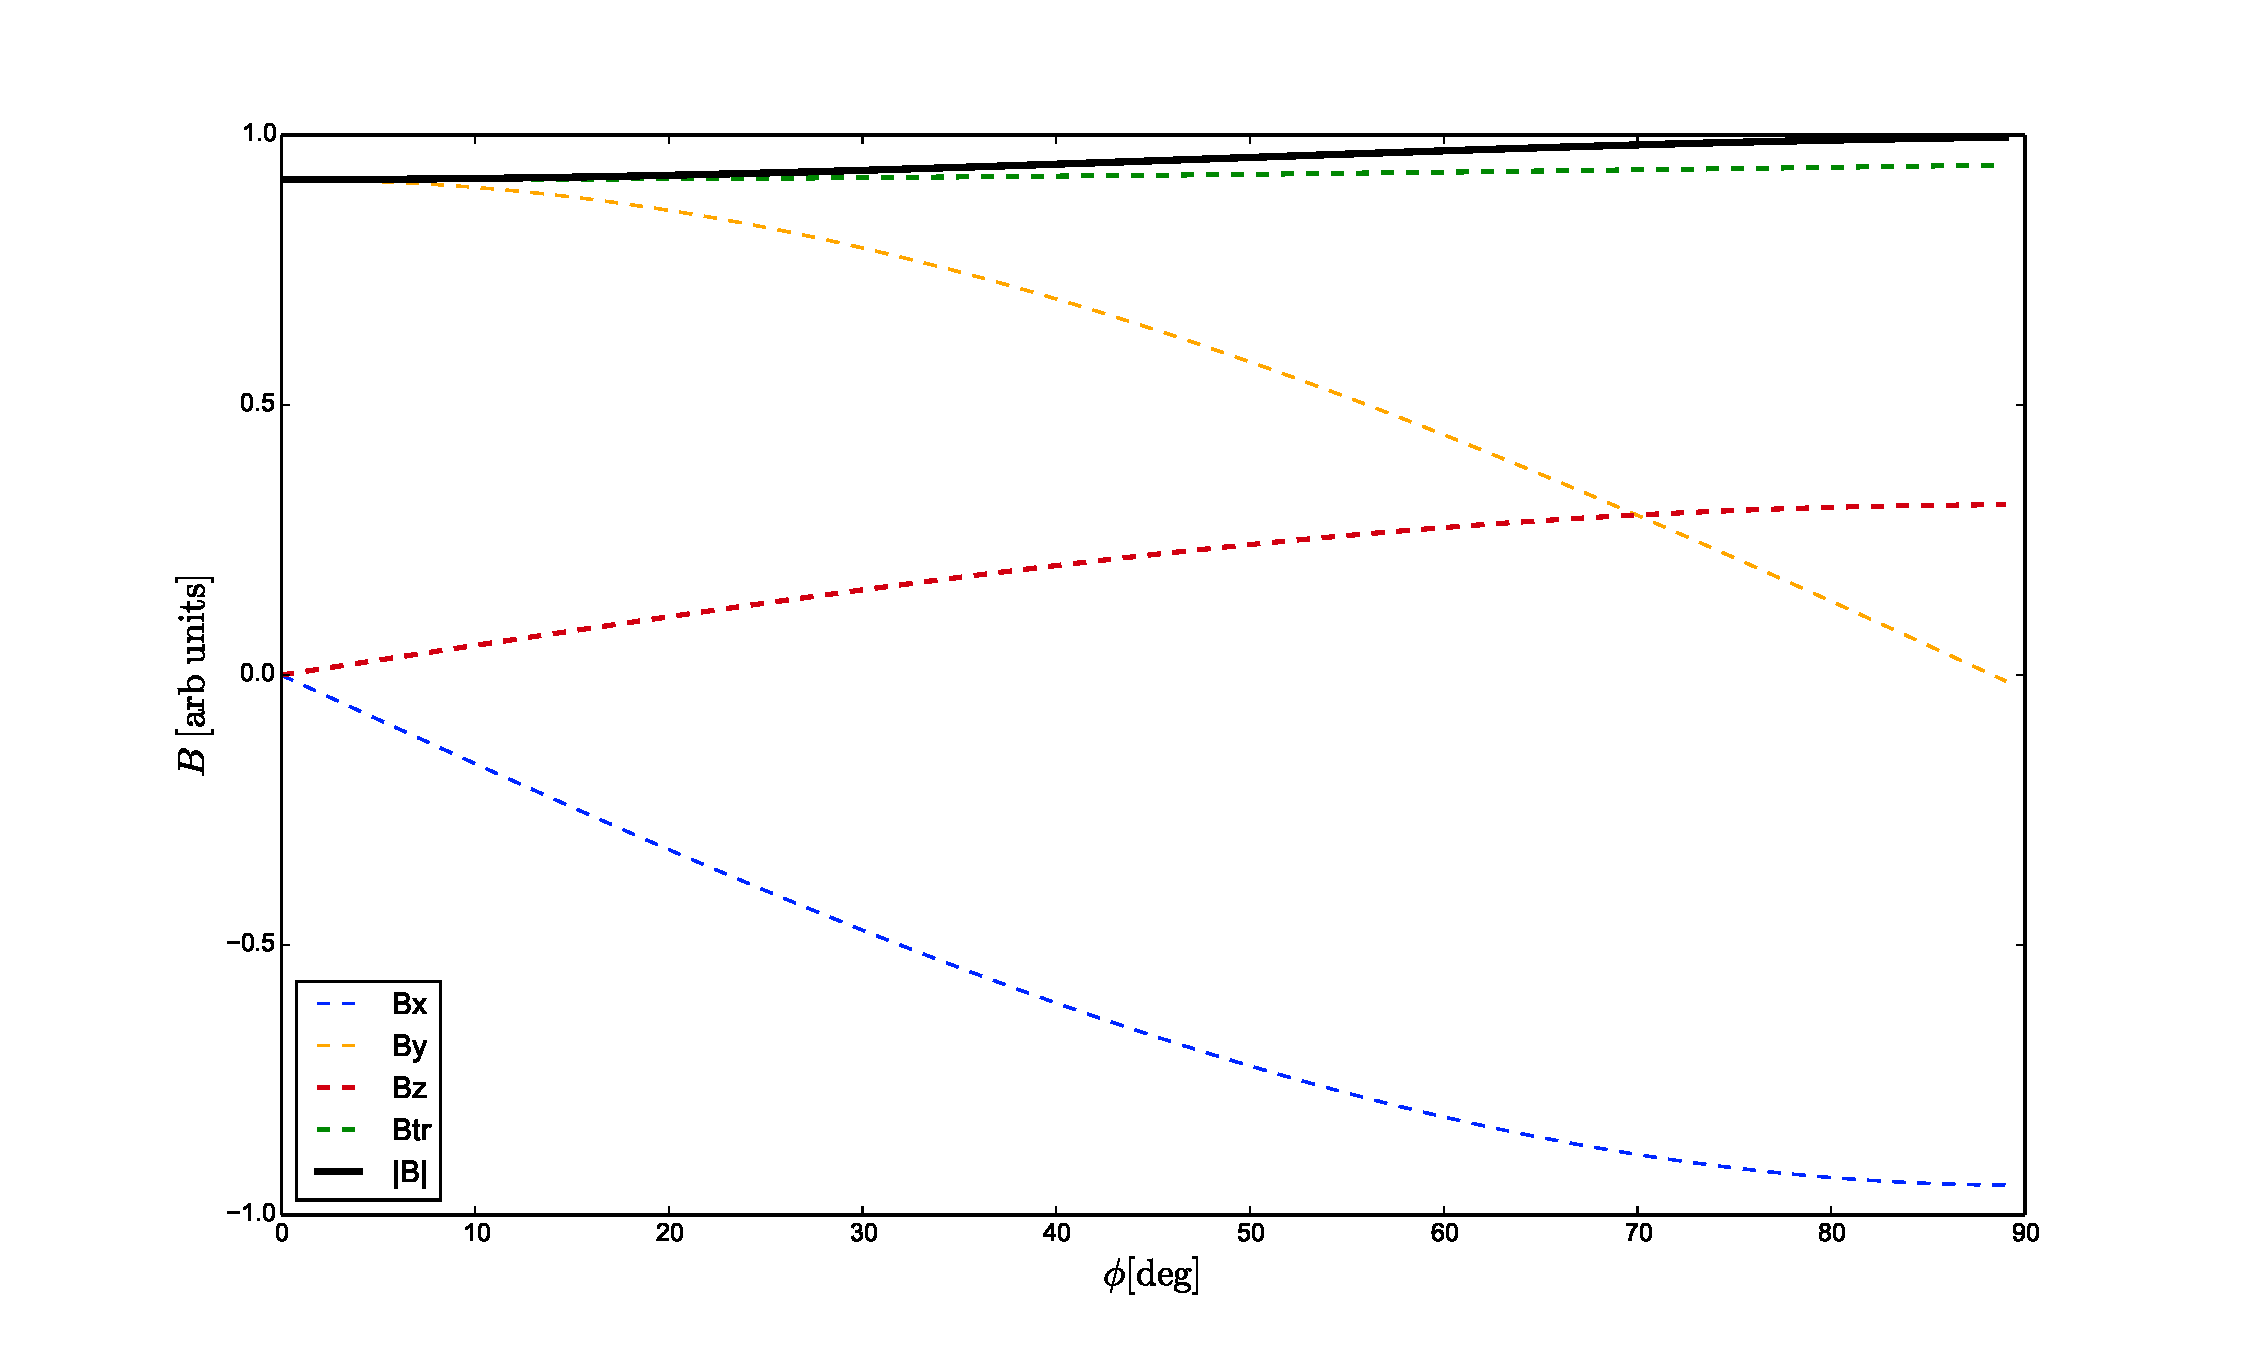
\includegraphics[width=\textwidth]{./fig/EASRadio/geomComps_Tunka}
		\caption{\label{fig:geomComps_Tunka}
		asd
		}
	\end{figure}
	
	\begin{figure}[ht!]
		\centering
		\includegraphics[width=\textwidth]{./fig/simulacionRadio/{ZHSEvent_18_89.5_0_25_On_1238_E}.png}
		\includegraphics[width=\textwidth]{./fig/simulacionRadio/{ZHSEvent_18_89.5_0_25_Off_1238_E}.png}
		\caption{\label{fig:testFootprint_Ez}
		asd
		}
	\end{figure}
	
	\begin{figure}[ht!]
		\centering
		\includegraphics[width=\textwidth]{./fig/simulacionRadio/{ZHSEvent_18_89.5_0_25_On_1238_Ey}.png}
		\includegraphics[width=\textwidth]{./fig/simulacionRadio/{ZHSEvent_18_89.5_0_25_Off_1238_Ey}.png}
		\caption{\label{fig:testFootprint_Ez}
		asd
		}
	\end{figure}
	
	\begin{figure}[ht!]
		\centering
		\includegraphics[width=\textwidth]{./fig/simulacionRadio/{ZHSEvent_18_89.5_0_25_On_1238_Ez}.png}
		\includegraphics[width=\textwidth]{./fig/simulacionRadio/{ZHSEvent_18_89.5_0_25_Off_1238_Ez}.png}
		\caption{\label{fig:testFootprint_Ez}
		asd
		}
	\end{figure}
	
		\begin{figure}[ht!]
		\centering
		\includegraphics[width=\textwidth]{./fig/simulacionRadio/{ZHSEvent_18_89.5_0_25_On_1238_Ex}.png}
		\includegraphics[width=\textwidth]{./fig/simulacionRadio/{ZHSEvent_18_89.5_0_25_Off_1238_Ex}.png}
		\caption{\label{fig:testFootprint_Ez}
		asd
		}
	\end{figure}
	
	Bon y Boff
	
	mostrar que los efectos son comparables.
	
	velocidad de drift peque\~na por alra densidad en la atmosfera.
	
	\clearpage
	\subsection{Distribuci\'on de part\'iculas vs. se\~nal de radio}
	
	remarcar que el footprint es mucho mas extenso que la distribucion de particulas
	
	\begin{figure}[ht!]
		\centering
		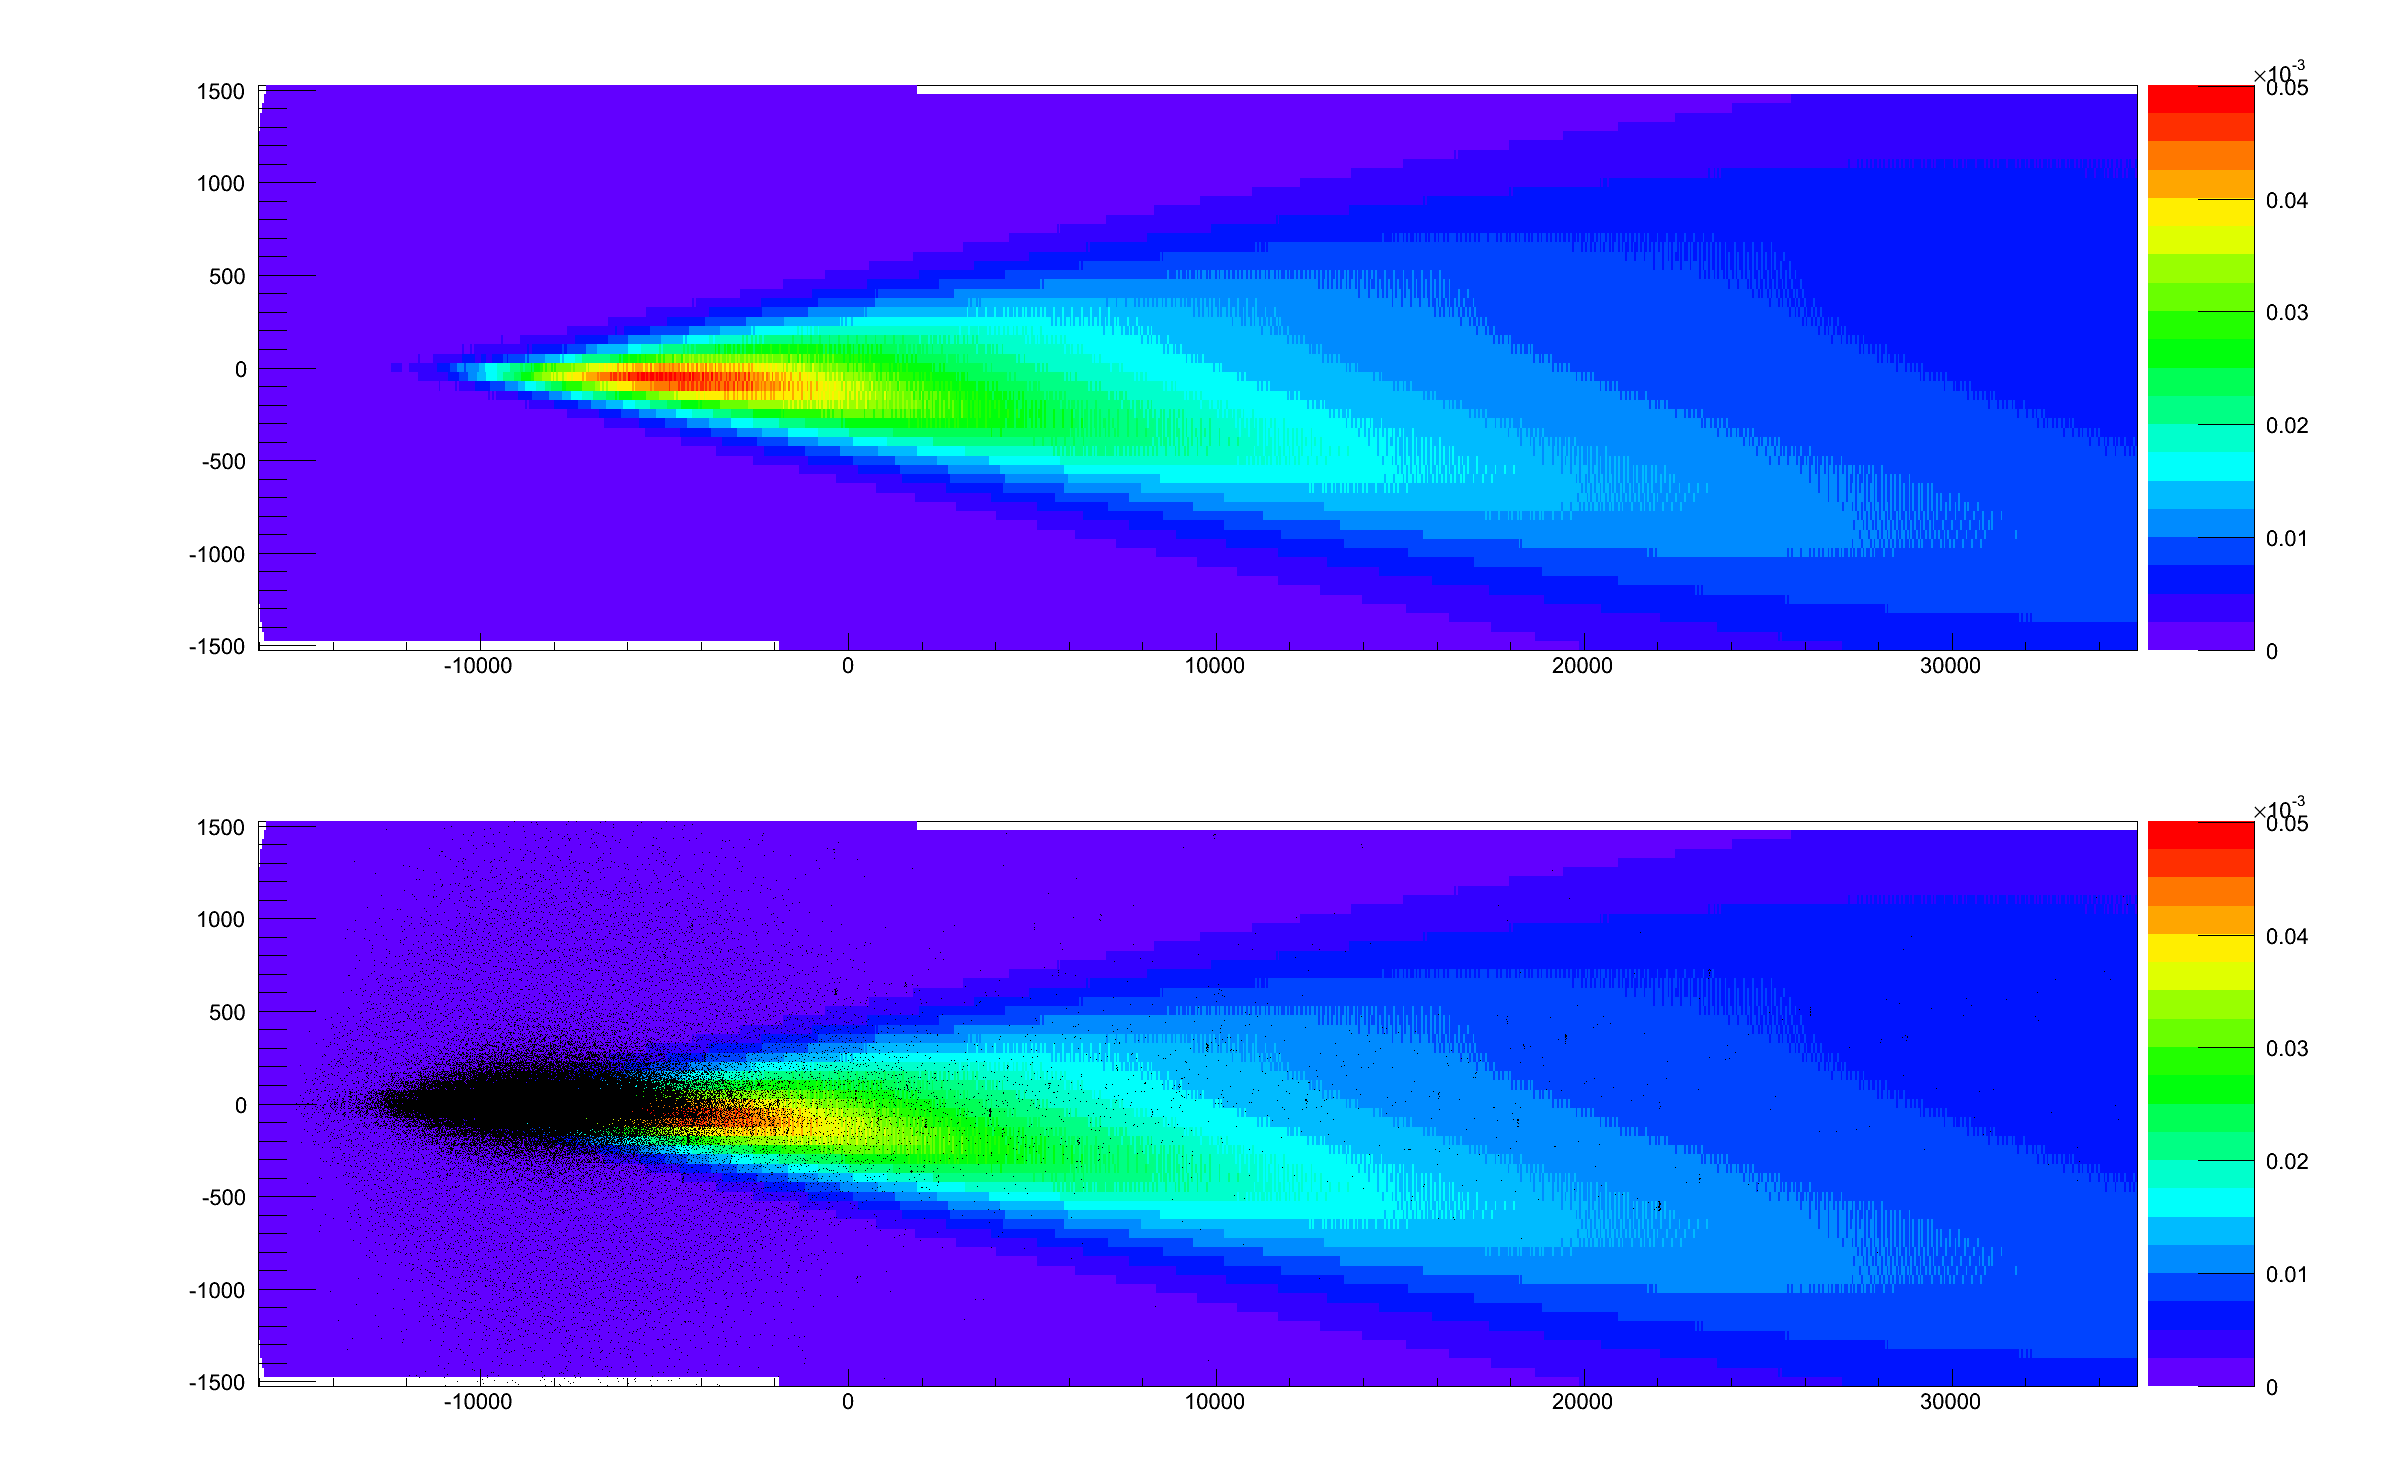
\includegraphics[width=0.8\textwidth]{./fig/simulacionRadio/ZHSEvent_1238_denseArray_E_Particulas}
		\caption{\label{fig:sim_foot_y_part}
		asd
		}
	\end{figure}
	
	\subsection{Dependencia con el canal de decaimiento del \tauon{}}
	
	Graficar distribuciones de diferentes variables que importen para diferentes canales.
	
	Energia visible
	Ancho de la lluvia
	Maximo del footprint
	
	
	

